%!TEX root = ../main.tex

\chapter{Sistemi Dinamici} % (fold)
\label{cha:sistemi_dinamici}

Un modello matematico per descrivere le dinamiche di un sistema non lineare è lo spazio degli stati. Con questo modello si pensa in termini di variabili di stato i cui valori ad un certo istante temporale sono considerati sufficienti a predire la futura evoluzione del sistema.\\

Sia $\bar{x}(t) = x_1(t), \dots, x_N(t)$ il \textbf{vettore di stato}, un vettore contenente le variabili di stato di un sistema dinamico non lineare, in cui la variabile indipendente è il tempo $t$ e $N$ è l'ordine del sistema. È possibile allora descrivere un largo numero di sistemi dinamici non lineari mediante un sistema di equazioni differenziali di primo ordine chiamate equazioni dello spazio degli stati ed aventi la seguente forma:
\begin{align}
	\frac{d}{dt} \bar{x}(t) = F(\bar{x}(t))\label{eq:stati}
\end{align}
dove $F(\bar{x})$ è una funzione vettore che se applicata ad un vettore $\bar{x}$ ritorna un vettore che ha come j-esima componente $F_j(x_j)$ con $F_j$ una qualche funzione; si può pensare a quest'ultimo come come ad un \textbf{vettore di velocità}. Un sistema in cui la funzione vettore $F$ non dipende esplicitamente dal tempo è detto \textbf{autonomo}. In questo capitolo saranno trattati solo sistemi dinamici autonomi.\\

L'Equazione~\eqref{eq:stati} può essere vista come un descrittore del movimento di un punto nello spazio degli stati N-dimensionale; questo punto non è altro che lo stato del sistema osservato ad un certo istante $t$. Con lo scorrere del tempo il punto $t$ descrive una curva nello spazio degli stati detta \textbf{traiettoria} o orbita del sistema.

\newpage

La velocità istantanea della traiettoria è rappresentata da un vettore tangente; possiamo quindi derivare un vettore di velocità per ogni punto della traiettoria.
La famiglia delle traiettorie, per differenti condizioni iniziali, è chiamato \emph{ritratto degli stati} del sistema e comprende tutti quei punti per cui $F(\bar{x})$ è definita; nel caso di sistemi autonomi per ogni punto dello spazio esiste una sola traiettoria che vi passa.

\begin{figure}[h!]
	\centering
	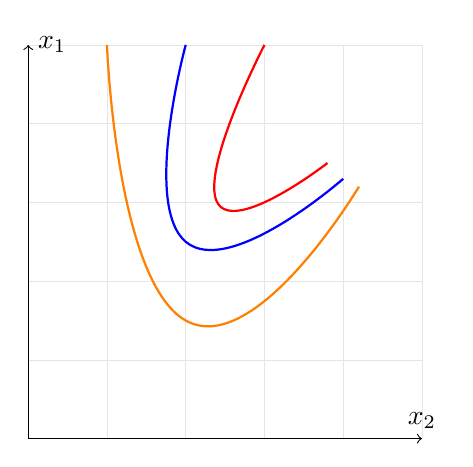
\begin{tikzpicture}
	    \draw[very thin,color=gray!20] (0,0) grid (5,5);
	    \draw[->] (0,0) -- (0,5) node[right] {$x_1$};
	    \draw[->] (0,0) -- (5,0) node[above] {$x_2$};

	    \draw[thick, color=red] plot [smooth, tension=1] coordinates{(3, 5) (2.4, 3) (3.8, 3.5)};
	    \draw[thick, color=blue] plot [smooth, tension=1] coordinates{(2, 5) (2, 2.5) (4, 3.3)};
	    \draw[thick, color=orange] plot [smooth, tension=1] coordinates{(1, 5) (2, 1.5) (4.2, 3.2)};
	\end{tikzpicture}
	\caption{Un ritratto degli stati bidimensionale di un sistema dinamico.}
\end{figure}

\section{Condizione di Lipschitz} % (fold)
\label{sub:condizione_di_lischitz}
Affinchè l’equazione dello spazio degli stati abbia soluzione e questa sia unica è necessario imporre alcune restrizioni sul vettore $F(\bar{x})$. Condizione sufficiente affinchè vi sia soluzione è che $F(x)$ sia continua in tutti i suoi argomenti; tuttavia questa condizione non garantisce l’unicità della soluzione. Serve una restrizione più forte conosciuta come condizione di Lipschitz. Una funzione:
\begin{align*}
    \mathbf{f}: \Omega \subseteq \mathbb{R}^n \rightarrow \mathbb{R}^m
\end{align*}
si dice “lipschitziana” su $\Omega$ se:
\begin{align*}
    \exists K \ge 0 
\end{align*}
tale che 
\begin{align*}
    \left \| \mathbf{f}(\mathbf{x}) - \mathbf{f}(\mathbf{y}) \right \| \le K \left \| \mathbf{x} - \mathbf{y} \right \| \qquad \forall \mathbf{x}, \mathbf{y} \in \Omega 
\end{align*}

\newpage

\begin{figure}[h!]
    \centering
    \begin{tikzpicture}[domain=-2:2]
        \begin{axis}[restrict y to domain=-2:2, grid]
            \addplot[blue,smooth,thick] function{sin(x) * cos(4 * x)} node[above=1cm] {\tiny$\sin(x)\cos(4x)$};
            \addplot[green, thick] function{- 4 * x} node[below] {\tiny$-4x$};
            \addplot[green, thick] function{4 * x} node[above] {\tiny$4x$};
        \end{axis}
    \end{tikzpicture}
    \caption{Interpretazione grafica della Condizione di Lipschitz: la funzione $f=\sin(x)\cos(4x)$ è lipschitziana con $K=4$. Ciò significa che se si considera un qualunque punto lungo la funzione e si tracciano le rette di coefficienti angolari 4 e -4, allora $f$ non sarà mai confinata tra le due rette.}
\end{figure}

% section condizione_di_lischitz (end)

\section{Stati di equilibrio} % (fold)
\label{sub:stabilità_degli_stati_di_equilibrio}
Intuitivamente un punto/stato di equilibrio stabile è un punto che non risente delle piccole perturbazioni: se ci si sposta poco da un punto stabile il sistema continuerà a rimanere anche in futuro nelle vicinanze di quel punto. L'esempio più semplice è quello di una pallina disposta esattamente nel fondo di una valle, se la spostiamo di poco dal fondo può rotolare in basso ed oscillare ma non aumenta la sua distanza dal punto di equilibrio.\\

Viceversa un punto di equilibrio instabile è tale per cui basta una perturbazione arbitrariamente piccola dall'equilibrio per far allontanare significativamente il sistema dalla posizione iniziale. Un esempio è una pallina disposta sulla cima di una collina.\\

Un vettore costante $\bar{x}\in M$ è detto stato di equilibrio (stazionario) se è soddisfatta la seguente condizione:
\begin{align*}
    \mathbf{F}(\bar{x}) = 0
\end{align*}
dove 0 è il vettore nullo. Il vettore velocità si annulla nel punto di equilibrio e quindi $\mathbf{x}(t) = x$ è una soluzione dell'equazione dello spazio degli stati. Lo stato di equilibrio è anche detto punto singolare e la traiettoria degenera nel punto stesso. Si enunciano ora una serie di definizioni sulla stabilità degli stati di equilibrio.

\begin{mydef}
    Lo stato di equilibrio $x$ è detto \textbf{uniformemente stabile} se per ogni $\bar{x}$ positivo, esiste un $\epsilon$ positivo tale che la condizione:
    \begin{align*}
        \left|\mathbf{x}(0) - \bar{x} \right| < \delta
    \end{align*}
    implica
    \begin{align*}
        \left|\mathbf{x}(t) - \bar{x} \right| < \epsilon
    \end{align*}
    per ogni $t > 0$.
\end{mydef}

Questa definizione afferma che una traiettoria del sistema può essere fatta stare in un piccolo
intorno dello stato di equilibrio $\bar{x}$ se il suo stato iniziale è vicino a $\bar{x}$.

\begin{mydef}
    Lo stato di equilibrio $x$ è detto \textbf{convergente} se esiste un $\delta$ positivo tale che la
    condizione:
    \begin{align*}
        \left|\mathbf{x}(0) - \bar{x} \right| < \delta
    \end{align*}
    implica che:
    \begin{align*}
        \lim_{t \rightarrow \infty} \mathbf{x}(t) = \bar{x}
    \end{align*}
\end{mydef}
Questa seconda definizione afferma che se lo stato iniziale di una traiettoria è adeguatamente vicino allo stato di equilibrio $x$, allora la traiettoria descritta dal vettore di stato $x(t)$ convergerà a $x$ all'aumentare del tempo.
% section stabilità_degli_stati_di_equilibrio (end)
\begin{mydef}
    Lo stato di equilibrio $\bar{x}$ è detto \textbf{asintoticamente stabile} se è stabile e convergente.
\end{mydef}
\begin{mydef}
    Lo stato di equilibrio $x$ è detto \textbf{globalmente asintoticamente stabile} se è stabile e se
    tutte le traiettorie del sistema convergono a $x$ per $t$ che tende ad infinito.
\end{mydef}

\newpage


\section{Teorema di Lyapunov} % (fold)
\label{sub:teorema_di_lyapunov}
Si enunciano ora i due teoremi di Lyapunov che forniscono condizioni sufficienti per l'esistenza di un punto stazionario.

\begin{thm}[Primo teorema di Lyapunov]
    Lo stato di equilibrio $\bar{x}$ è stabile se in un piccolo intorno di $\bar{x}$ esiste una funzione definita positiva $V(x)$ tale che la sua derivata rispetto al tempo è minore o uguale a 0 in quella regione.
\end{thm}

\begin{thm}[Secondo teorema di Lyapunov]
     Lo stato di equilibrio $\bar{x}$ è asintoticamente stabile se in un piccolo intorno di $\bar{x}$ esiste una funzione definita positiva $V(x)$ tale che la sua derivata rispetto al tempo sia strettamente minore di 0 in quella regione.
\end{thm}

Una funzione scalare $V(x)$ che soddisfa queste proprietà è detta \textbf{funzione di Lyapunov} per lo stato di equilibrio $\bar{x}$.
La funzione $V(x)$ è definita positiva nello spazio degli stati $L$, se $\forall x \in L$, soddisfa le seguenti proprietà:
\begin{enumerate}
    \item la funzione $V(x)$ ha derivate parziali rispetto agli elementi di $\mathbf{x}$ continue;
    \item $V(\bar{x})=0$;
    \item $V(x)>0$ se $\mathbf{x} \neq \bar{x}$.
\end{enumerate}

Supposta $V(x)$ una funzione di Lyapunov, lo stato di equilibrio $\bar{x}$ è stabile se:
\begin{align*}
    \frac{d}{dt} \cdot V(\mathbf{x}) \leq 0, \qquad \text{se } \left|x - \bar{x} \right| \leq \epsilon
\end{align*}
dove $\epsilon$ è un numero positivo. Lo stato di equilibrio è asintoticamente stabile se:
\begin{align*}
    \frac{d}{dt} \cdot V(\mathbf{x}) < 0, \qquad \text{se } \left|x - \bar{x} \right| \leq \epsilon
\end{align*}

Il criterio è una generalizzazione del fatto, ben noto nella fisica, che un sistema meccanico, se lasciato libero di evolvere, tende a portarsi in una configurazione dove la sua energia potenziale è minima. La funzione di Lyapunov può quindi essere interpretata come una funzione di energia potenziale generalizzata. Il criterio dice che uno stato di equilibrio è stabile se:
\begin{enumerate}
    \item è minimo per una certa funzione di energia generalizzata (cioè se esiste una funzione di Lyapunov definita positiva);
    \item se il sistema tende a portarsi verso la configurazione di minimo della funzione di Lyapunov (cioè se la derivata della funzione di Lyapunov è semidefinita negativa).
\end{enumerate}
Il criterio è una \textbf{condizione sufficiente ma non necessaria}. Non è detto in generale che l'origine non sia stabile se non esiste una funzione di Lyapunov definita in un intorno dell'origine. Inoltre non esiste un algoritmo per trovare la funzione di Lyapunov relativa a un sistema, ma si deve cercare per tentativi, basandosi sul tipo di funzione di stato e su considerazioni puramente fisiche.

% section teorema_di_lyapunov (end)
% chapter sistemi_dinamici (end)
